\documentclass{article}
\usepackage{ifplatform}

\ifmacosx
\usepackage[fontset=mac]{ctex}
\fi
\iflinux
\usepackage[fontset=ubuntu]{ctex}
\fi

\usepackage{amsmath}
\usepackage{amssymb}
\usepackage{graphicx}

% http://kuing.orzweb.net/viewthread.php?tid=3004
\newcommand\rsx[1]{\left.{#1}\vphantom{\big|}\right|}

\title{Homework 2 - Credit Card\\ Default Payment Prediction}
\author{資工系博士班二年級 D06922023 顏志軒}

\begin{document}

\maketitle

\textbf{Problem 1.} (1\%) 請簡單描述你實作之 logistic regression 以及 generative model 於此 task的表現,試著討論可能原因。

\textbf{Problem 2.} (1\%) 請試著將 input feature 中的 gender, education, martial status 等改為 one-hot encoding 進行 training process,比較其模型準確率及其可能影響原因。

\textbf{Problem 3.} (1\%) 請試著討論哪些 input features 的影響較大(實驗方法不限)。

\textbf{Problem 4.} (1\%) 請實作特徵標準化 (feature normalization),討論其對於你的模型準確率的影響。

\textbf{Problem 5.} (1\%) The Normal (or Gaussian) Distribution is a very common continuous probability distribution. Given the PDF of such distribution

\begin{equation}
f(x) = \frac{1}{\sqrt{2\pi}\sigma}e^{-\frac{(x-\mu)^2}{2\sigma^2}}, -\infty < x < \infty
\end{equation}

please show that such integral over $(-\infty, \infty)$ is equal to 1.

所求的值為:

\begin{equation}
\int_{-\infty}^{\infty}\frac{1}{\sqrt{2\pi}\sigma}e^{-\frac{(x-\mu)^2}{2\sigma^2}}dx
\end{equation}

令此值為$I$。此時$I^2$的值為:

\begin{equation}\label{square}
\begin{aligned}
I^2
=&\left(\int_{-\infty}^{\infty}\frac{1}{\sqrt{2\pi}\sigma}e^{-\frac{(x-\mu)^2}{2\sigma^2}}dx\right)^2\\
\=&\left(\int_{-\infty}^{\infty}\frac{1}{\sqrt{2\pi}\sigma}e^{-\frac{(x-\mu)^2}{2\sigma^2}}dx\right) \left(\int_{-\infty}^{\infty}\frac{1}{\sqrt{2\pi}\sigma}e^{-\frac{(y-\mu)^2}{2\sigma^2}}dy\right)\\
=&\int_{-\infty}^{\infty}\int_{-\infty}^{\infty}\frac{1}{2\pi\sigma^2}e^{-\frac{(x-\mu)^2+(y-\mu)^2}{2\sigma^2}}dx dy
\end{aligned}
\end{equation}

令$x=\mu+\sigma r \textrm{cos}\theta, y=\mu+\sigma r \textrm{sin}\theta$,則$dx dy=\sigma^2 r dr d\theta$,方程式\ref{square}可變換為:

\begin{equation}\label{polar}
I^2=\int_{0}^{2\pi}\int_{0}^{\infty}\frac{1}{2\pi}e^{-\frac{r^2}{2}}rdrd\theta
\end{equation}

接著,令$t=e^{-\frac{r^2}{2}}$,則$dt=-re^{-\frac{r^2}{2}}dr$,方程式\ref{polar}成為:

\begin{equation}
\begin{aligned}
I^2
=&\int_{0}^{2\pi}\rsx{-\frac{1}{2\pi}e^{-\frac{r^2}{2}}}_{0}^{\infty}d\theta\\
=&\int_{0}^{2\pi}\frac{1}{2\pi}d\theta\\
=&\rsx{\frac{\theta}{2\pi}}_{0}^{2\pi}\\
=&1
\end{aligned}
\end{equation}

由於$f(x)$在整個實數軸皆為正數,因此I也是正數,即為1。

\textbf{Problem 6.} (1\%) Given a three layers neural network, each layer labeled by its respective index variable. I.e. the letter of the index indicates which layer the symbol corresponds to.

\begin{center}
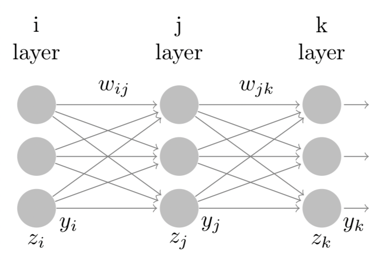
\includegraphics{network}
\end{center}

For convenience, we may consider only one training example and ignore the bias term.Forward propagation of the input $z_i$ is done as follows. Where $g(z)$ is some differentiable function (e.g. the logistic function).

\begin{equation*}
\begin{aligned}
y_i = g(z_i)\\
z_j = \sum_{i}^{}w_{ij}y_i\\
y_j = g(z_j)\\
z_k = \sum_{j}^{}w_{jk}y_j\\
y_k = g(z_k)
\end{aligned}
\end{equation*}

Derive the general expressions for the following partial derivatives of an error function $E$, also sime differentiable function, in the feed-forward neural network depicted. In other words, you should derive these partial derivatives into "computable derivative" (e.g., $\frac{\partial E}{\partial y_k}$ or $\frac{\partial z_k}{\partial w_{jk}}$).
\begin{center}
(a) $\frac{\partial E}{\partial z_k}$
(b) $\frac{\partial E}{\partial z_j}$
(c) $\frac{\partial E}{\partial w_{ij}}$
\end{center}

\end{document}
